\chapter{Representações gráficas}
\label{sec:graf}
\section*{Como fazer um histograma}
\label{sec:histo}

Quando fazemos uma análise estatística de um conjunto de $N$ medidas de uma determinada grandeza, podemos realizar um gráfico no qual se representa para cada valor (ou intervalo de valores) o número de vezes em que este aparece. Este tipo de gráfico recebe o nome de {\bf Histograma}. Um exemplo é mostrado na Figura~\ref{fig:histo}. Como o conjunto de valores obtidos é discreto, resulta um esquema de barras. A largura destas barras é a menor diferença entre os valores medidos ou o tamanho do intervalo escolhido no caso em que seja conveniente agrupar vários valores num intervalo (isto deve ser determinado em função da série de medições realizadas). O número de barras depende do conjunto de dados e do número total de medições. 

\begin{figure}[h]
\begin{center}
\vspace{-1.5cm}
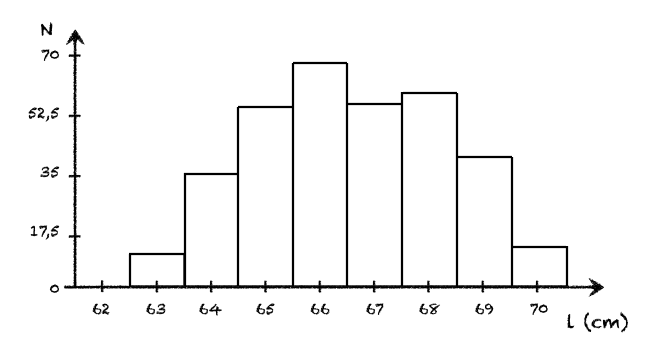
\includegraphics[width=12cm]{fig/HistogramWhite}
\vspace{-0.7cm}
\caption{\label{fig:histo} Exemplo de um histograma.}
\vspace{-1.cm}
\end{center}
\end{figure}
%-___ fim

Para que fique mais claro, vamos considerar o seguinte exemplo.  Medimos a altura de uma garrafa de água 40 vezes obtendo os seguintes valores, em centímetros:

\begin{center}
\hspace{-0.8cm}
  \begin{tabular}[m]{c c c c c c c c}
 20,3	 & 20,1 & 20,2 & 20,5 & 20,2 & 19,7 & 20,6 & 20,4\\
 19,8 & 20,3 & 20,1 & 20,2 & 20,3 & 20,4 & 20,3 & 19,6\\
 20,0 & 19,5 & 20,7 & 20,3 & 20,1 & 20,7 & 20,5 & 20,5\\
 20,5 & 20,3 & 20,4 & 20,2 & 20,3 & 20,2 & 20,6 & 20,8\\
 20,4 & 20,0 & 19,9 & 20,6 & 20,8 & 19,7 & 20,9 & 20,3\\
  \end{tabular}
\end{center}
\vspace{-0.3cm}

Como podemos ver, há valores que se repetem e a frequência de repetição é diferente para cada valor. Esta informação pode ser apresentada em forma gráfica, mediante a construção de um histograma. Para isto devemos escolher valores ou intervalos de valores e determinar quantas vezes o valor se repete no conjunto de dados.

Para nosso exemplo, vamos escolher intervalos de 0,2 cm começando pelo menor valor medido de 19,5 cm.  Desta forma o primeiro intervalo será de 19,5 a 19,7 cm, o segundo de 19,7 cm a 19,9 cm e assim sucessivamente.  Cada intervalo será representado no gráfico pelo seu valor central, ou seja, para o primeiro será 19,6 cm, para o segundo 19,8 cm, etc.  Como os intervalos são contínuos devemos escolher como serão os limites dos intervalos, aberto e fechado, pois, por exemplo, o valor 19,7 cm vai contar para o primeiro ou o segundo intervalo. No nosso exemplo, o valor inferior vai ser o fechado e o valor superior o aberto (ou seja, 19,7 cm vai contar para o segundo intervalo e não para o primeiro). Desta forma, podemos construir a Tabela~\ref{tab:freq}, de frequências:
\begin{table}[!htbp]
\begin{center}
\hspace{-0.8cm}
\caption{Tabela de frequências absolutas e relativas em função da altura medida de uma garrafa.}\label{tab:freq}
  \begin{tabular}[m]{|c| c| c| c|}
  Intervalo (cm) & Valor do Intervalo (cm)	& Frequência & Frequência Relativa (\%)  \\
19,5 - 19,7	&	19,6	&	2   & 5,0 \\
19,7 - 19,9	&	19,8	&	3   & 7,5\\
19,9 - 20,1 	&	20,0	&	3   & 7,5\\
20,1	- 20,3	&	20,2	&	7   & 17,5\\
20,3 - 20,5	&	20,4	&	12 & 30,0\\
20,5 - 20,7	&	20,6	&	8   & 20,0\\
20,7 - 20,9	&	20,8	&	4   & 10,0 \\
20,9	- 21,1	&	21,0	&	1   &  2,5\\ 	
  \end{tabular}
\end{center}
\end{table}
\vspace{0.3cm}

Uma vez construída a tabela, podemos fazer o gráfico no qual vamos colocar no eixo-x os valores centrais dos intervalos escolhidos e no eixo-y o número de repetições (Frequência). Para isto deve ser escolhida uma escala adequada em cada eixo, de forma que a distância entre todos os valores centrais dos intervalos seja constante.  Para o caso do eixo-y, a escala deve ser escolhida de forma tal que o valor mais repetido fique na parte superior do eixo, de forma que possa ser apreciada a estrutura do histograma. Uma vez escolhida a escala, uma barra será desenhada para cada intervalo com o tamanho da frequência determinada na tabela anterior, como mostramos no lado esquerdo da Figura~\ref{fig:histoexemplo}.

Uma forma alternativa de se fazer o histograma é colocando no eixo-y a frequência relativa, ou seja, o número de repetições dividido pelo número total de medidas, frequentemente mostrado em percentagem, como na última coluna da Tabela~\ref{tab:freq} e no histograma do lado direito da Figura~\ref{fig:histoexemplo}. 

\begin{figure}[h]
\begin{center}
\begin{tabular}{cc}
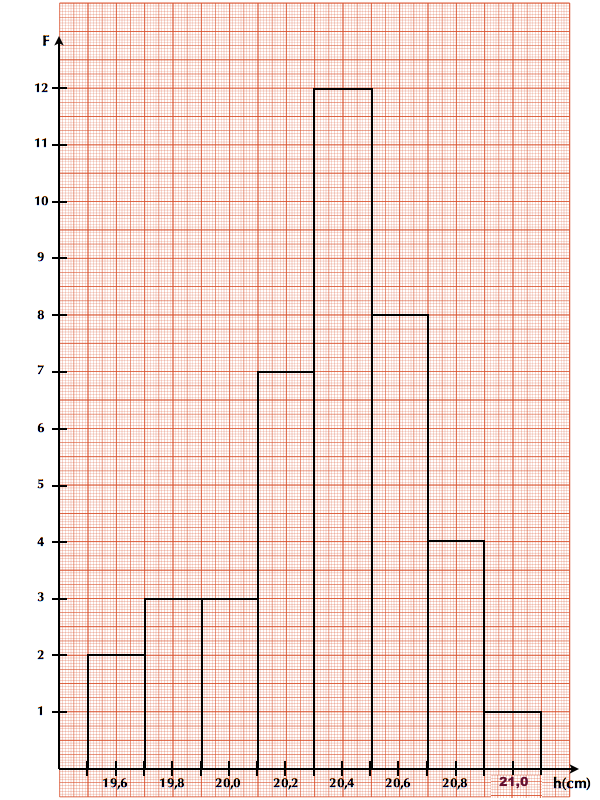
\includegraphics[width=8cm]{fig/histoH}&
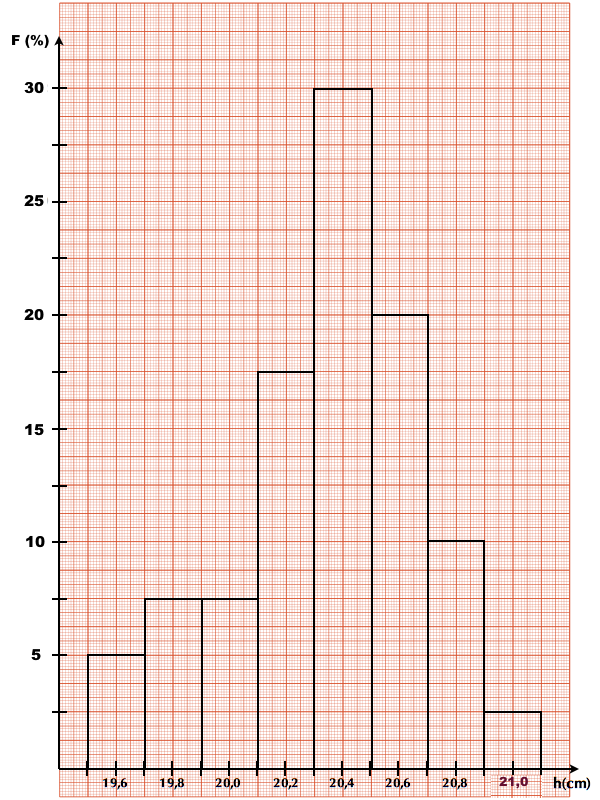
\includegraphics[width=8cm]{fig/histoHFR}\\
\end{tabular}
\caption{\label{fig:histoexemplo} Histogramas de frequências (lado esquerdo) e frequências relativas (lado direito) da medida da altura (h) da garrafa de água .}
\vspace{-1.cm}
\end{center}
\end{figure}



\section*{Como construir um gráfico}\label{plot}

Uma forma muito útil de apresentar os resultados experimentais é a partir de re\-pre\-sen\-ta\-ções gráficas dos mesmos, pois neles a informação é sintetizada, facilitando sua análise e interpretação. Geralmente, um gráfico é mais útil que uma tabela de valores, por exemplo, quando estamos realizando medições de uma variável Y em função de outra X que varia independentemente e queremos ver a relação funcional entre elas (por exemplo, a posição de um móvel em função do tempo), ou para estudar se duas variáveis possuem alguma correlação ou não.

Em Física Experimental I, todos os gráficos que realizaremos serão em duas dimensões além dos histogramas que já foram discutidos na sessão~\ref{sec:histo}. O primeiro passo é escolher quais serão as variáveis e, logo, qual é a variável independente que será representada no eixo horizontal e qual a dependente no eixo vertical.  Por exemplo, se queremos representar a posição de um corpo em movimento em função do tempo vamos identificar duas variáveis:  posição ($x$) e tempo (t), sendo o tempo a variável independente.  Ou seja, o tempo será colocado no eixo-x e a posição no eixo-y. 

Uma vez escolhidas as variáveis, devemos determinar a escala para cada eixo. Para isto temos que considerar os valores medidos de cada variável, de forma a poder escolher uma escala que facilite a leitura dos pontos experimentais, ou qualquer outro ponto representado no gráfico.  Quando desenhamos o gráfico em papel, devemos escolher a escala de forma a usar pelo menos metade da folha para representar os pontos experimentais. Para facilitar a leitura do gráfico, é interessante utilizar escalas em que cada milímetro do papel corresponda a múltiplos ou submúltiplos de 2 ou 5 da grandeza correspondente. A determinação da escala em cada eixo é independente.   

Consideremos os seguintes valores medidos para o exemplo da posição do corpo em função do tempo: %(Tabela~\ref{tab:dados}).
\vspace{-0.7cm}
\begin{center}
  \begin{tabular}{|c|c|c|}
  Tempo (s) & Posição (m)  & Incerteza da Posição (m)	\\
0,1	&	29 & 1 \\
0,3	&	34 & 1 \\
0,4	&	41 & 1 \\
0,5	&	38 & 1 \\ 
0,7	&	33 & 1 \\ 
1,0	&	26 & 1 \\
1,1	&	23 & 1 \\
1,2	&	20 & 1 \\
1,4	&	17 & 1 \\
1,5	&	16 & 1 \\
\end{tabular}
%\caption{Tabela da posição em função do tempo.
%\label{tab:dados} %}
\vspace{-0.4cm}
\end{center}

Vamos construir o gráfico em papel milimetrado, usando a folha ``na vertical'', de forma que o eixo-x fique na menor dimensão da mesma e o eixo-y na maior. Para o eixo-x, onde vamos representar o tempo, a escolha parece simples, começamos em 0 (zero) e consideramos uma escala de 10 mm para cada 0,1 s, pois o tamanho nesta dimensão é de 180 mm e nós precisamos marcar de 0 a 1,5 s. Para o eixo-y, onde vamos representar a posição, dispomos de 28 cm de folha. Neste caso, podemos considerar duas possibilidades: (A) começamos a escala a partir do zero ou (B) começamos ela perto do menor valor medido, neste caso 16 m.  Em ambos  os casos a escala deve ir até o máximo valor medido ou algum valor superior imediato.  Em geral escolhemos um valor superior que permita ajustar a escala para um múltiplo de 2 ou 5. Se consideramos o caso (A), uma escala possível seria 1 cm no papel para cada 2 m de posição (Figura~\ref{fig:plots} (esquerda)). Como podemos ver, não é necessário começar do zero, podemos começar por exemplo de 15 m (caso B) e escolher uma escala de 1 cm para cada 1 m (Figura~\ref{fig:plots} (direita)). Desta forma podemos observar melhor a estrutura própria do gráfico. Uma vez definida a escala, marcamos valores regularmente espaçados nos eixos correspondentes e identificamos os eixos com as grandezas que estes representam, com suas respectivas unidades. Finalmente, desenha-se os  pontos com suas barras de erro de acordo com a tabela de dados, como pode se ver na Figura~\ref{fig:plots}. A barra de erro é a representação gráfica da incerteza. Assim, ela deve ser desenhada como uma reta que vai de um valor igual ao valor do ponto subtraído do valor de uma incerteza até o valor do ponto somado de uma incerteza.

Não existe uma única forma de representar os nossos dados.  No exemplo anterior, ambos os gráficos estão corretos. {\bf O importante é que se deve adotar uma “escala limpa e fácil de ser lida” de modo a que não seja necessário fazer cálculos para achar a localização dos pontos no gráfico. Se você precisar fazer muitos cálculos, algo está inadequado.}

\begin{figure}[t]
\vspace{0.5cm}
\begin{minipage}{\textwidth}
\begin{minipage}[t]{0.47\textwidth}
 \begin{center}
 \includegraphics*[width=0.99\textwidth]{fig/Plot1}
\end{center}
\end{minipage}
%\hspace{0.3cm}
\begin{minipage}[t]{0.47\textwidth}
\begin{center}
 \includegraphics*[width=0.99\textwidth]{fig/Plot2}
     \end{center}
   \end{minipage}
 \end{minipage}
\caption{\label{fig:plots}  Gráfico da posição (x) em função do tempo (s) para o caso A (esquerda). Gráfico da posição (x) em função do tempo (s) para o caso B (direita).}
\end{figure} 

